\chapter{LFT: Real Physics on the Lattice}\label{ch:realPhys}

We are now in a position to start tackling some real-world physics using the
methods of LFT. Nowadays lattice calculations inform many branches of particle
physics where ab initio, non-perturbative investigations are useful, for example
when computing CKM matrix elements, when exploring the QCD phase diagram at
low-to-moderate temperature near zero quark chemical potential, hadron
spectroscopy, or learning about the muon anomalous magnetic moment, just to name
a few applications.

\section{QCD thermodynamics}\label{sec:QCDtherm} 

This chapter focuses on the phenomenology I worked on as a postdoc in
Bielefeld, i.e. the phase diagram of QCD. There are many useful reviews
on the market, for instance Ref.~\cite{ding_thermodynamics_2015}.

In the following we will focus on $N_f=2+1$ QCD using HISQ fermions. We are
interested in nonzero $\mu$, which is not accessible directly by the lattice.
One possible strategy is to expand in small $\muh\equiv\mu/T$. For the
pressure, we find\footnote{Note that this combination on the LHS of 
\equatref{eq:pxpac} is unitless. This is because area has units
MeV$^{-2}$ and force has units MeV$^2$.}
\begin{equation}\label{eq:pxpac}
\frac{P}{T^4}=\sum_{ijk}\frac{1}{i!j!k!}\,\chi_{ijk}^{(u)(d)(s)}(T)\,
               \muh_u^i\,\muh_d^j\,\muh_s^k,
\end{equation}
where we have defined the {\it generalized
susceptibility}\index{generalized susceptibility}
\begin{equation}
\chi_{ijk}^{(u)(d)(s)}(T)
  \equiv\frac{\partial^{\,i+j+k}\,P/T^4}{\partial\muh_u^i\partial\muh_d^j
                                       \partial\muh_s^k}\Big|_{\muh=0}.
\end{equation}
Some example generalized susceptibilities could be
\begin{equation}
  \chi_2^u=\frac{\partial^2}{\partial\muh_u^2}\frac{P}{T^4}
  ~~~~\text{or}~~~~
  \chi_{11}^{us}=\frac{\partial^2}{\partial\muh_u\partial\muh_s}\frac{P}{T^4}.
\end{equation}

Another set of useful relations is between chemical potentials in the flavor
$(u,d,s)$ basis and the conserved charge $(B,Q,S)$ basis\footnote{Yet a further
possible basis of conserved charges is the $(B,I,S)$ basis with isospin $I\equiv I_3$.
For the purpose of distinguishing between $u$ and $d$ quarks only, one can use
either $I$ or $Q$.
To learn more in detail about isospin, see \secref{sec:isohyper}.}, i.e. the basis
of baryon number, electric charge, and strangeness. These relations 
are\footnote{A mnemonic to remember these relations is to ask what each quark
contributes to a system. For example a strange quark makes 1/3 of a baryon,
adds charge -1/3, and subtracts 1 from the strangeness.}
\begin{equation}\begin{aligned}\label{eq:quark-conservedCharge}
  \mu_u &= \frac{1}{3}\mu_B + \frac{2}{3}\mu_Q\\
  \mu_d &= \frac{1}{3}\mu_B - \frac{1}{3}\mu_Q\\
  \mu_s &= \frac{1}{3}\mu_B - \frac{1}{3}\mu_Q - \mu_S.
\end{aligned}\end{equation}
These relations are needed whenever one is interested in {\it conserved
charge fluctuations},\index{conserved charge fluctuation} i.e. susceptibilities like
\begin{equation}
\chi_{ijk}^{(B)(Q)(S)}(T)
  \equiv\frac{\partial^{\,i+j+k}\,P/T^4}{\partial\muh_B^i\partial\muh_Q^j
                                       \partial\muh_S^k}\Big|_{\muh=0}.
\end{equation}
Since none of the conserved charges appears directly in the action, one
instead must decompose a conserved charge derivative into quark derivatives
using \equatref{eq:quark-conservedCharge}. For example 
one finds
\begin{equation}
  \pdv{\mu_B}
   =\sum_f\pdv{\mu_f}{\mu_B}\pdv{\mu_f}
   =\frac{1}{3}\sum_f\pdv{\mu_f}.
\end{equation}

Now we will connect this to the partition function $Z$. We have
\begin{equation}
  \frac{P}{T^4}=\frac{1}{VT^3}\log Z,
\end{equation}
where as usual $V=(aN_s)^3$ and $T=1/aN_\tau$.
When there are $N_f$ flavors and when we use the HISQ action we have,
according to \equatref{eq:HISQdist},
\begin{equation}
  Z=\int\DD U\prod_f (\det D_f)^{1/4}\,e^{-S_G}
\end{equation}
and compute expectation values of the observable $X$ as
\begin{equation}\label{eq:HISQev}
  \ev{X}=\frac{1}{Z}\int\DD U\prod_f(\det D_f)^{1/4}\,e^{-S_G}X.
\end{equation}

Recall that in the grand canonical ensemble, a particle number
$N$ enters the Boltzmann factor as $\mu N$; so a particle number density 
for a quark flavor $f$ is extracted as\footnote{Remember that there is also
an overall $1/T$ factor in the exponent in natural units.}
\begin{equation}\label{eq:nfdensity}
  \frac{1}{V}\,\partial_{\muh_f}\log Z
  =\frac{1}{VZ}\,\partial_{\muh} Z
  =\ev{n_f}.
\end{equation}
In the staggered formulation, all the dependence on $\muh_f$ will be
hidden in $D_f$, so for $f\neq g$ we get
\begin{equation}
  \partial_{\muh_f}D_g = 0.
\end{equation}
Finally we note that, for the purpose of doing Taylor series expansions, it is
useful to remember that the QCD partition function should be blind to charge
conjugation at $\mu_B=0$. This tells us that we should expect only even powers
of $\mu_B$ when using that as the expansion parameter. 

\subsection{Derivative formulas}

We will now derive some formulas which are useful for calculations in QCD
thermodynamics. You can find even more useful formulas for a system of 
$N_f$ identical
fermion flavors in the appendix of Ref.~\cite{allton_thermodynamics_2005}.
For these calculations we will often need the following formula for an
invertible matrix $M$:
\begin{theorem}{The exp-trace-log (ETL) formula}{}\label{thm:exptrlog} 
  $$\det M = \exp \tr \log M$$
\end{theorem}
Let $M$ depend on $\alpha\in\C$ and let $y\in\R$. Then from the ETL formula
\begin{equation}\begin{aligned}
  \partial_\alpha(\det M)^y &= y(\det M)^{y-1}\partial_\alpha\det M\\
      &= y(\det M)^{y-1}\exp\left[\tr\log M\right]\partial_\alpha\tr\log M\\
      &= y(\det M)^y \tr M^{-1}\partial_\alpha M.
\end{aligned}\end{equation}
This formula is useful in evaluating derivatives of roots of the fermion
matrix determinant. A final formula useful for matrix derivatives is
\begin{equation}
  \partial_\alpha M^{-1} = - M^{-1}\left(\partial_\alpha M\right) M^{-1}.
\end{equation}

Our goal is to eventually take derivatives of expectation values, so from
\equatref{eq:HISQev} we will need $\muh$-derivatives of the partition 
function. For the following few formulas 
I will assume arbitrarily many non-degenerate
fermion flavors\footnote{I find this helpful to get prefactors that appear
in terms in, e.g., $\chi_2^u$ correct.}. Assuming $S_G$ has no 
$\muh$-dependence, we find
\begin{equation}
  \partial_{\muh}Z = \frac{1}{4}\sum_f 
                      Z\ev{\tr D_f^{-1}\partial_{\muh}D_f}.
\end{equation}
Hence 
\begin{equation}\label{eq:dZinv}
  \partial_{\muh}Z^{-1} = -Z^{-2}\partial_{\muh}Z
                        =\frac{1}{4}\sum_fZ\ev{\tr D_f^{-1}\partial_{\muh}D_f}
\end{equation}
and
\begin{equation}\label{eq:dlogZ}
  \partial_{\muh}\log Z=\frac{1}{4}\sum_f\ev{\tr D_f^{-1}\partial_{\muh}D_f}.
\end{equation}
Comparing \equatref{eq:dlogZ} with \equatref{eq:nfdensity} we find in
the staggered formulation
\begin{equation}
  n_f=\frac{1}{4V}\tr D_f^{-1}\partial_{\muh_f}D_f.
\end{equation} 
Finally using \equatref{eq:dZinv} one quickly derives the following useful formula
for an observable $O$ calculated on HISQ configurations:
\begin{proposition}{}{dO}
\begin{equation*} \partial_{\muh}\ev{O}
       =   \ev{\partial_{\muh}O}
        -\frac{1}{4}\sum_f\ev{\tr D_f^{-1}\partial_{\muh}D_f}\ev{O}
         +\frac{1}{4}\sum_f\ev{O\tr D_f^{-1}\partial_{\muh}D_f}
\end{equation*}
\end{proposition} 
Note that if $\muh=\muh_f$ with $N_f$ degenerate flavors, 
\propref{prp:dO} reduces to eq.~(A3)
in Ref.~\cite{allton_thermodynamics_2005}. Using this Proposition along
with \equatref{eq:dlogZ}, one 
can start expressing generalized susceptibilities in terms of the fermion
matrix. For example one finds for any flavor $f$
\begin{equation}\begin{aligned}
  VT^3\,\chi_2^f =\partial_{\muh_f}^{\,2}\log Z
                 =\, & \frac{1}{16}\ev{\left(\tr D_f^{-1}D_f'\right)^2}
                    -\frac{1}{16}\ev{\tr D_f^{-1}D_f'}^2\\
                   & -\frac{1}{4}\ev{\tr \left(D_f^{-1} D_f'\right)^2}
                    +\frac{1}{4}\ev{\tr D_f^{-1}D_f''},
\end{aligned}\end{equation}
where a prime on $D_f$ indicates a derivative w.r.t. the corresponding chemical
potential $\muh_f$. Similarly for two flavors $f\neq g$ 
\begin{equation}\begin{aligned}
  VT^3\,\chi_{11}^{fg} =\partial_{\muh_f}\partial_{\muh_g}\log Z
                 = \,& \frac{1}{16}\ev{\tr D_f^{-1}D_f'\tr D_g^{-1}D_g'} \\
                   & -\frac{1}{16}\ev{\tr D_f^{-1}D_f'}\ev{\tr D_g^{-1}D_g'}.
\end{aligned}\end{equation}
Using an $N_f=2+1$ HISQ action with $m_l\equiv m_u=m_d$ along with 
\equatref{eq:quark-conservedCharge}, one can figure out how to 
express\footnote{Note that when carrying out calculations like these, to avoid making mistakes,
one should always work with non-degenerate flavors, then allow the flavors to be
degenerate at the end. This way one correctly distinguishes between e.g.
$\chi_{11}^{ll}$ and $\chi_2^l$.} conserved charge fluctuations in terms of 
generalized susceptibilities, such as
\begin{equation}
  \chi_2^B=\frac{1}{9}\left(2\chi_2^l+\chi_2^s+2\chi_{11}^{ll}+4\chi_{11}^{ls}\right)
\end{equation}
and
\begin{equation}
  \chi_2^Q=\frac{1}{9}\left(5\chi_2^l+\chi_2^s-4\chi_{11}^{ll}-2\chi_{11}^{ls}\right).
\end{equation}


\subsection{Dealing with the sign problem}\index{sign problem}

\begin{figure}
\centering
\vspace{-1cm}
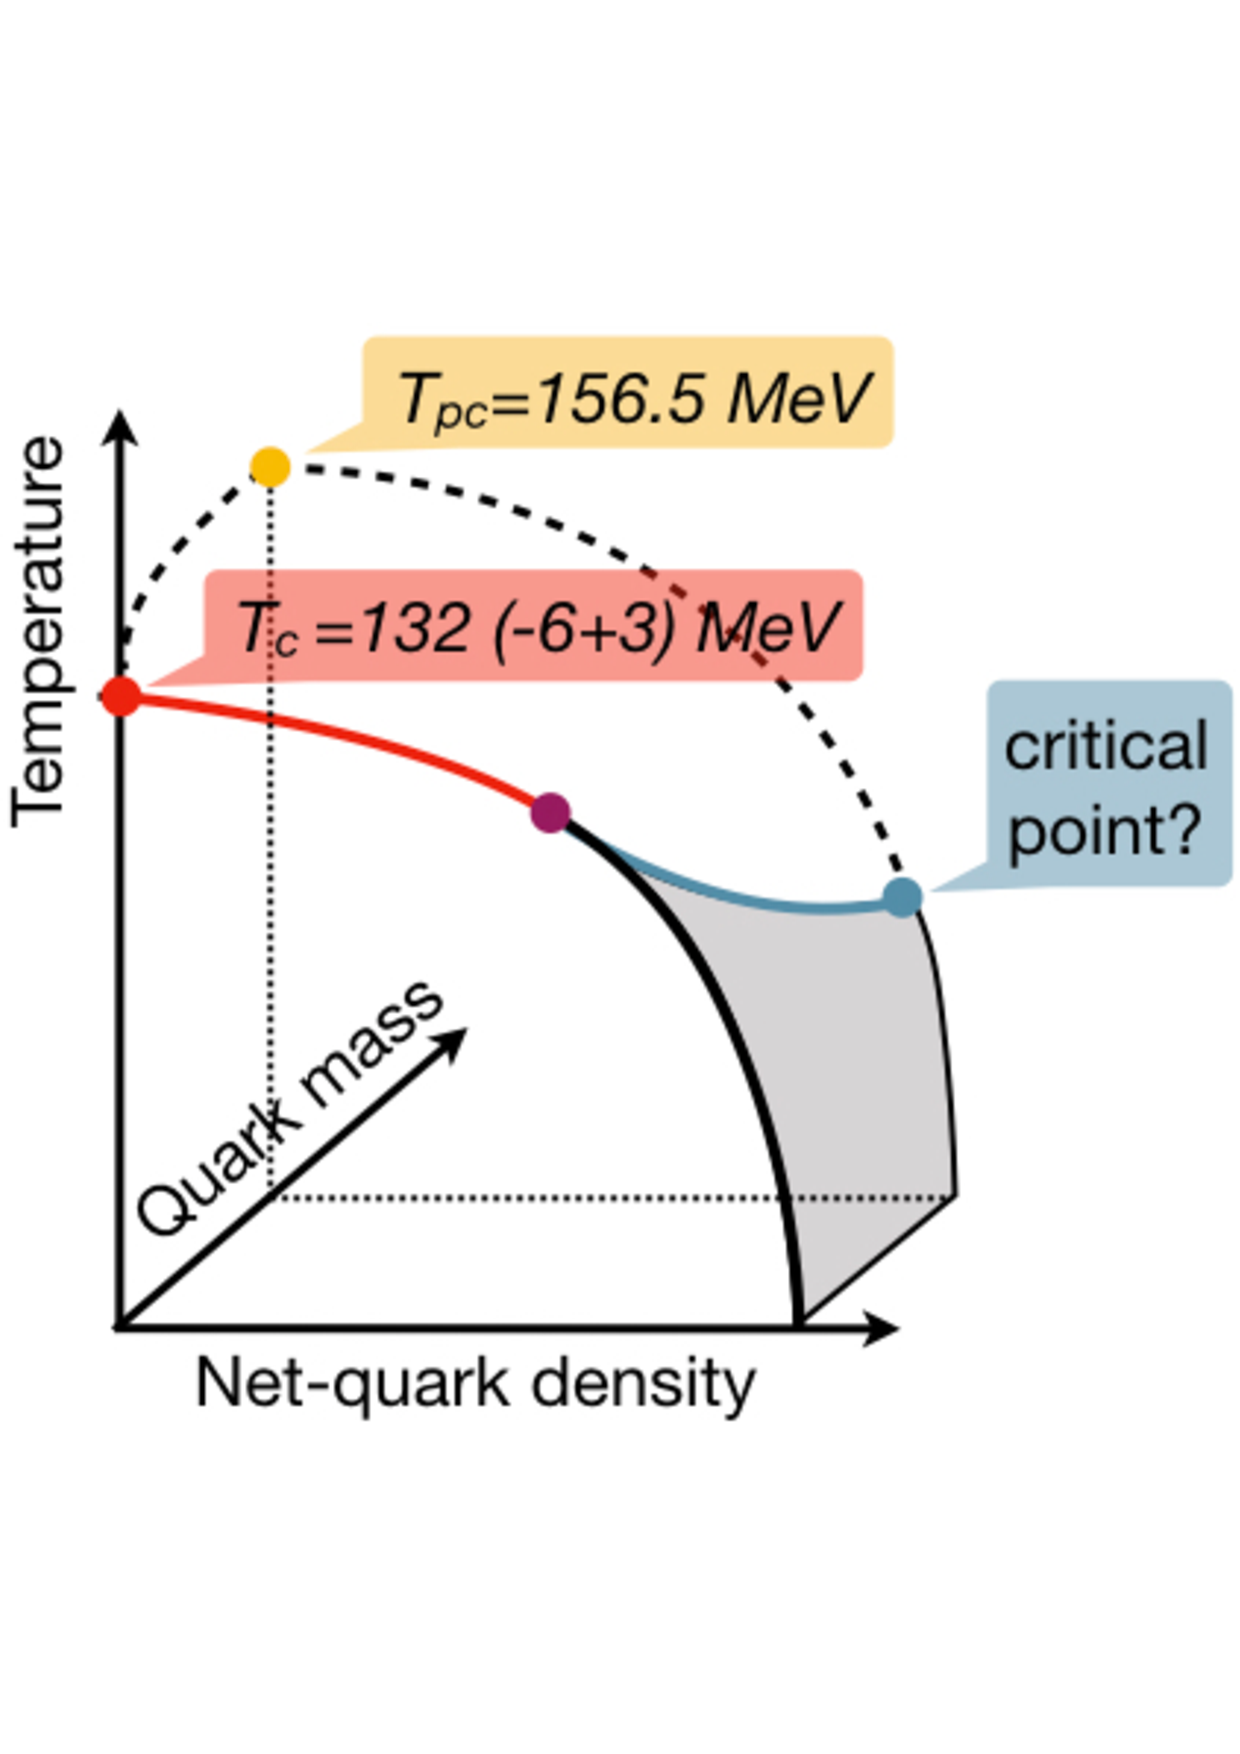
\includegraphics[width=0.4\linewidth]{figs/3d_phase_diag_Gauss.003.pdf}
\vspace{-1cm}
\caption{Schematic phase diagram of QCD. Indicated are the pseudocritical transition temperature 
$\Tpc$ of QCD at physical quark mass and the critical transition temperature $\Tc$ in the 
chiral limit. Dashed lines indicate crossovers, thick, solid lines are lines of second-order phase 
transitions, and a first-order surface is indicated in grey. A possible critical endpoint 
is indicated in teal. Figure by C. Schmidt.}
\label{fig:pdiag}
\end{figure}

At sufficiently high $T$ and/or $\mu_B$, nucleons dissociate into their constituents, 
and nuclear matter changes phase from a gas of hadrons to quark-gluon plasma.
At low enough temperature, one eventually encounters with increasing $\mu_B$ a line of 
first-order transitions, which is expected to terminate at a second-order critical 
endpoint belonging to the 3-$d$, $\Z_2$ universality class, as shown in the rear 
plane of Fig.~\ref{fig:pdiag}.


Unfortunately at $\mu_B>0$, the Boltzmann factor becomes complex, and a direct estimate of the path 
integral through MCMC is no longer possible--this is the infamous {\it sign problem}.
This limitation is a special hindrance when looking out for the possible critical 
endpoint at nonzero $\mu_B$ mentioned above. 
Nevertheless many approaches have been developed to at least partially circumvent this limitation, 
each with its own merits, drawbacks, and regions of applicability.
Two popular approaches include Taylor expansions of the equation of state in 
$\muh\equiv\mu_B/T$~\cite{Allton:2002zi, Allton:2003vx, Gavai:2003mf} and analytic continuation 
from purely imaginary chemical potential  $\muh=i\muh_I$~\cite{deForcrand:2002hgr, DElia:2002tig}.

When viewed from the plane of complex $\muh$, the Taylor expansion approach is limited by the 
location of the nearest zero of the QCD partition function $\ZQCD$, i.e. the nearest singularity 
of the free energy in the complex plane. 
In terms of the universal scaling in the vicinity of a critical point, the nearest singularity 
might be identified with the Lee-Yang edge\index{Lee-Yang singularity} 
singularity~\cite{yang_statistical_1952,lee_statistical_1952}, which is a branch cut 
singularity of the universal scaling function \cite{fonseca_zamolodchikov}. 
Two of these (complex conjugated) singularities pinch the real axis as $T$ approaches its 
critical value $\Tc$. The extended analyticity conjecture (due to Fonseca and Zamolodchikov) 
posits that, for $T < \Tc$, the Lee-Yang edge singularities are the closest singularities to 
the real axis of the symmetry breaking field $H$.
Thus understanding the analytic structure of the QCD free energy gives crucial insight on both
the convergence radius of these $\muh$-expansions and universal critical behaviour 
in the vicinity of the phase transitions.

\subsection{Speed of sound}

%In this section, we follow the introductions of Ref.~\cite{He:2022kbc}
%and Ref.~\cite{sorensen_speed_2021}, which have
%a lot of good references and context for calculating the speed of sound in QCD
%matter.

The speed of sound at fixed control parameter $X$ is defined as
\begin{equation}
  c_X^2=\left(\pdv{p}{\epsilon}\right)_X.
\end{equation}
In a simple (1+1)-$d$ isotropic model of a heavy ion collision, 
sometimes referred to as \index{Bjorken flow}{\it Bjorken flow}, 
assuming a constant $c_s^2$, one can show~\cite{bjorken_highly_1983} 
that the energy density will decrease with proper time $\tau$ as
\begin{equation}
  \epsilon(\tau)=\epsilon(\tau_0)\left(\frac{\tau_0}{\tau}\right)^{1+c_s^2}.
\end{equation}
In this picture one thus finds the system cools with longitudinal expansion
of the fireball according to the speed of sound. % Henrik's thesis is nice
Also in the context of heavy ion collisions, it can be used to look out
for a long-lived fireball, which may coincide with a {\it softest point}
\index{softest point} where the pressure-to-energy-density ratio,
and hence $c_s^2$, attains a minimum~\cite{hung_hydrodynamics_1995}.
In the context of neutron stars, $c_s^2$ is interesting since the relationship
between the star masses and radii is influenced by how $c_s^2$ changes with
$n_B$~\cite{ozel_masses_2016}.

The speed of sound has been calculated at $\mu_B=0$ on the 
lattice~\cite{borsanyi_qcd_2010,bazavov_equation_2014,borsanyi_full_2014}.
It has also been calculated using PNJL and NJL 
\index{NJL model}\index{PNJL model}
models\footnote{The Nambu-Jona-Lasinio (NJL)
model~\cite{nambu_dynamical_1961,nambu_dynamical_1961-1} is a low-energy,
effective model of interacting chiral fermions, i.e. it has a 4-fermion
interaction term. This means it's non-renormalizable, so it is not expected
to be a correct description at very high energies.
In the Polyakov-loop-extended NJL (PNJL) model~\cite{meisinger_chiral_1996}, 
one includes the zeroth component of the gauge field. The field is assumed to
be spatially uniform.}~\cite{ghosh_susceptibilities_2006,marty_transport_2013,deb_estimating_2016,motta_isentropic_2020,zhao_thermodynamic_2020};
in the quark-meson coupling
model~\cite{schaefer_thermodynamics_2010,abhishek_transport_2018};
the field correlator
method~\cite{khaidukov_speed_2018,khaidukov_thermodynamics_2019};
and in the quasiparticle method~\cite{mykhaylova_impact_2021}.


\bibliographystyle{unsrtnat}
\bibliography{bibliography}
